\chapter{Caso de uso concreto}

En este capítulo se introducirá un caso de uso concreto del sistema ARgos, mediante fotos del
sistema real funcionando. Además, se detallará cada imagen para dar a conocer el estado en qué se
encuentra el sistema en ese momento.

\section{Prerrequisitos}

La Figura~\ref{fig:ARgos_hardware} muestra los componentes hardware empleados por la unidad de
detección y despliegue. Previo inicio del sistema, el usuario cuenta con dos facturas que utilizará
en esta demostración. Además, cada factura lleva asociada un \textit{script} que será ejecutado una
vez el sistema detecte la factura correspondiente.

\section{Carga del sistema}

Durante la carga del sistema, el registro de eventos muestra por la salida especificada los sucesos
correspondientes al cliente y el servidor durante esa etapa (véase Figura~\ref{fig:Client_init} y
Figura~\ref{fig:Server_init}, respectivamente). Para el cliente (y detallando el registro
correspondiente a ARgos), el registro muestra que la conexión con el servidor se ha realizado
correctamente, la inicialización del contexto OpenGL ES y la carga de imágenes que se usarán más
tarde por el sistema. Para el caso del servidor, el registro muestra la carga en memoria de los
\textit{scripts} y la IP y el puerto donde está escuchando conexiones de clientes.

Arrancado el sistema, el proyector muestra una imagen cargada desde disco por ARgos con
información sobre un supuesto usuario ficticio (véase Figura~\ref{fig:ARgos_intro}).

\section{Bucle principal}

Pasado un tiempo (por defecto 10 segundos), el sistema avanza hacia el próximo estado en que entra
en el bucle principal de detección de documentos, delegación de tareas y renderizado. Este estado es
fácilmente reconocible por proyectar las cuatro esquinas del área de trabajo sobre la superficie
(véase Figura~\ref{fig:ARgos_waiting}).

En este caso, el usuario coloca el primer documento sobre la superficie de trabajo comprendida entre
las cuatro esquinas. Tras esto, el sistema renderiza varios componentes gráficos correspondientes a
ese documento. Además, se presentan varios botones que el usuario puede pulsar para iniciar un vídeo
que traduce a lengua de signos el documento. (véase Figura~\ref{fig:ARgos_facture1}).

Después, el usuario coloca el segundo documento. Para este caso, el sistema renderiza varios
componentes gráficos correspondientes a ese documento (véase
Figura~\ref{fig:ARgos_facture2}). Además, se presentan varios botones que el usuario puede pulsar
para ver de forma ampliada al darle la vuelta al documento, una imagen sobre lo que este ha marcado
en el propio documento (véase Figura~\ref{fig:ARgos_facture2_1}).

Para el tercer documento, está definido que se inicie una videollamada al darle la vuelta al
documento si se pulsa uno de los botones (véase Figura~\ref{fig:ARgos_facture3}). La
Figura~\ref{fig:ARgos_videostream2} muestra como se han empezado a recibir fotogramas del servidor y
son renderizados sobre el propio documento junto a una imagen de fondo.

Volviendo al registro de eventos, la Figura~\ref{fig:Client_loop} y la
Figura~\ref{fig:Server_listening} muestran respectivamente los registros de eventos del cliente y
del servidor mientras se ejecuta el bucle principal del sistema.

Finalmente, la Figura~\ref{fig:Client_release} muestra el cierre del cliente de manera limpia
liberando la memoria del sistema y cerrando los subsistemas adecuados.

\begin{figure}[!h]
  \begin{center}
    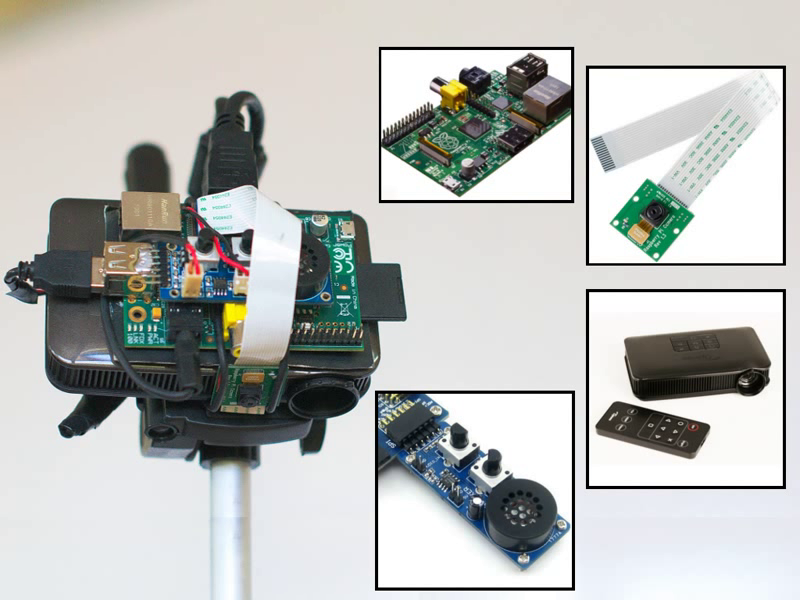
\includegraphics[width=1.0\textwidth]{ARgos_hardware.png}
    \caption{Hardware de ARgos.}
    \label{fig:ARgos_hardware}
  \end{center}
\end{figure}

\begin{figure}[!h]
  \begin{center}
    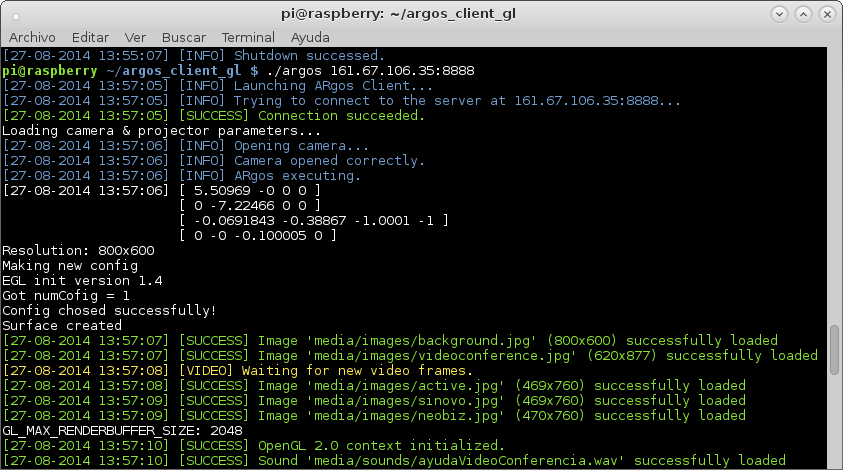
\includegraphics[width=1.0\textwidth]{Client_init.png}
    \caption{Inicialización del cliente.}
    \label{fig:Client_init}
  \end{center}
\end{figure}

\begin{figure}[!h]
  \begin{center}
    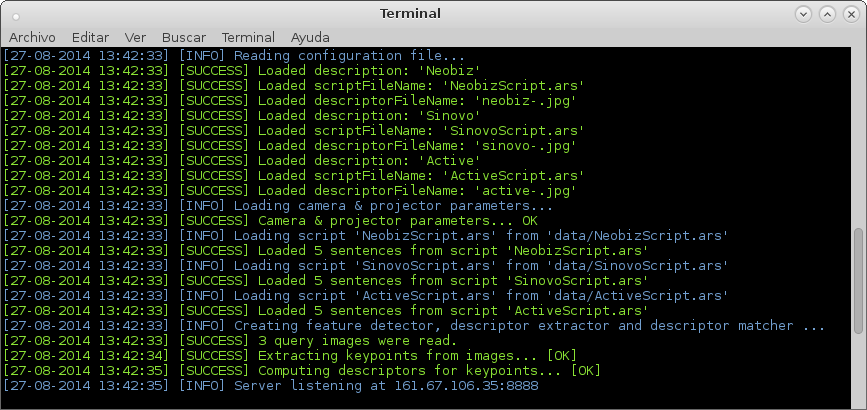
\includegraphics[width=1.0\textwidth]{Server_init.png}
    \caption{Inicialización del servidor.}
    \label{fig:Server_init}
  \end{center}
\end{figure}

\begin{figure}[!h]
  \begin{center}
    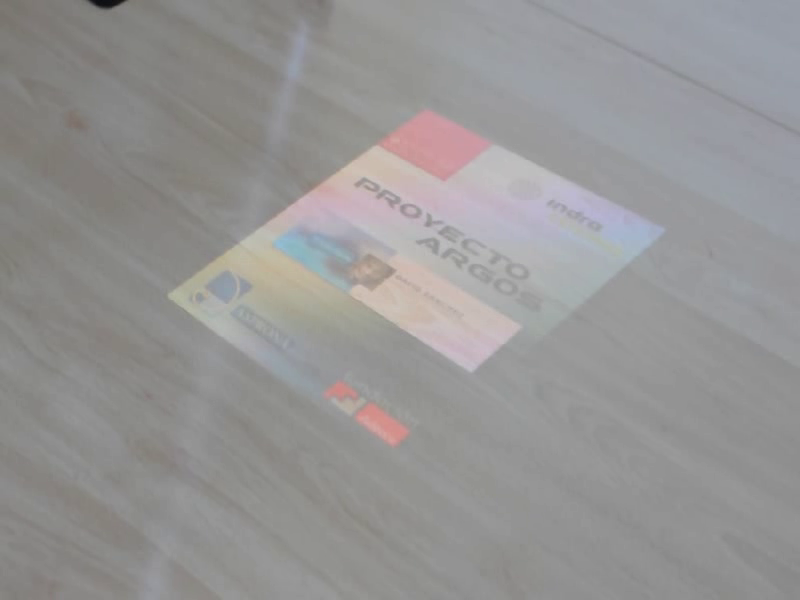
\includegraphics[width=1.0\textwidth]{ARgos_intro.png}
    \caption{Arranque de ARgos.}
    \label{fig:ARgos_intro}
  \end{center}
\end{figure}

\begin{figure}[!h]
  \begin{center}
    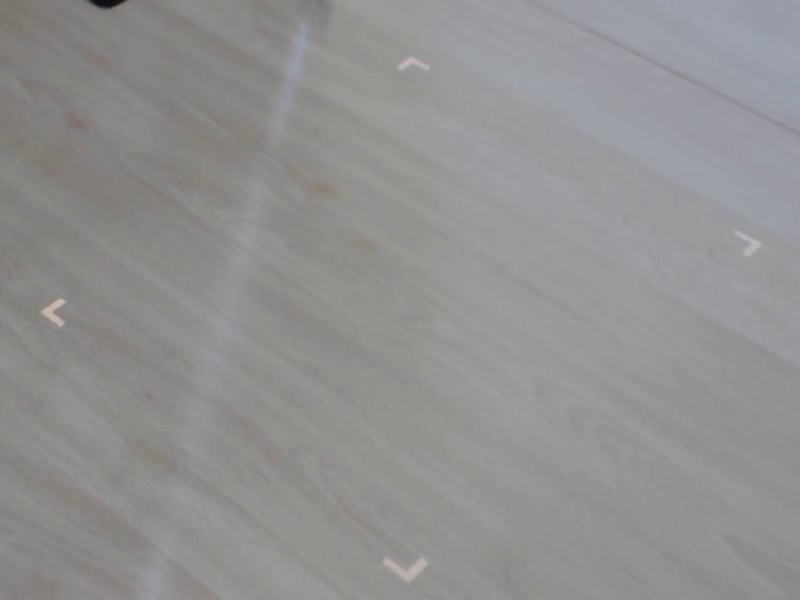
\includegraphics[width=1.0\textwidth]{ARgos_waiting.png}
    \caption{ARgos esperando por documentos.}
    \label{fig:ARgos_waiting}
  \end{center}
\end{figure}

\begin{figure}[!h]
  \begin{center}
    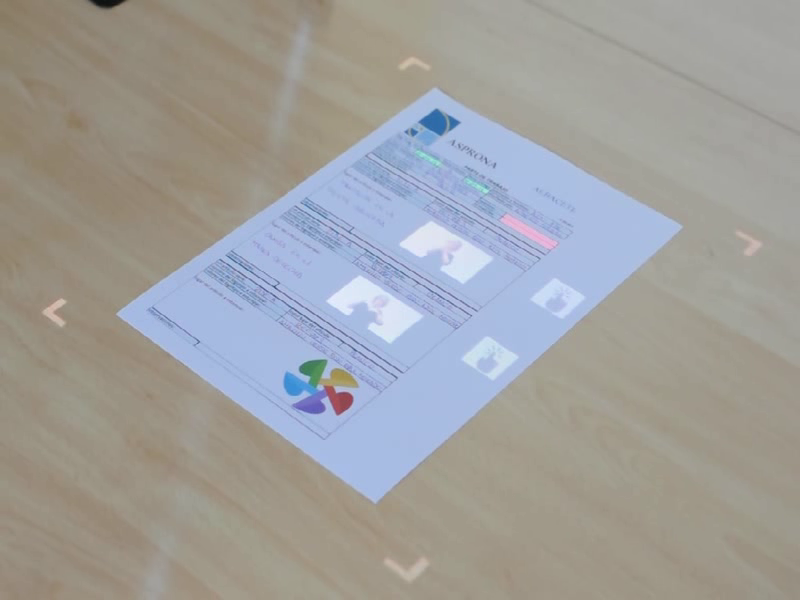
\includegraphics[width=1.0\textwidth]{ARgos_facture1.png}
    \caption{Primer documento detectado y componentes gráficos desplegados.}
    \label{fig:ARgos_facture1}
  \end{center}
\end{figure}

\begin{figure}[!h]
  \begin{center}
    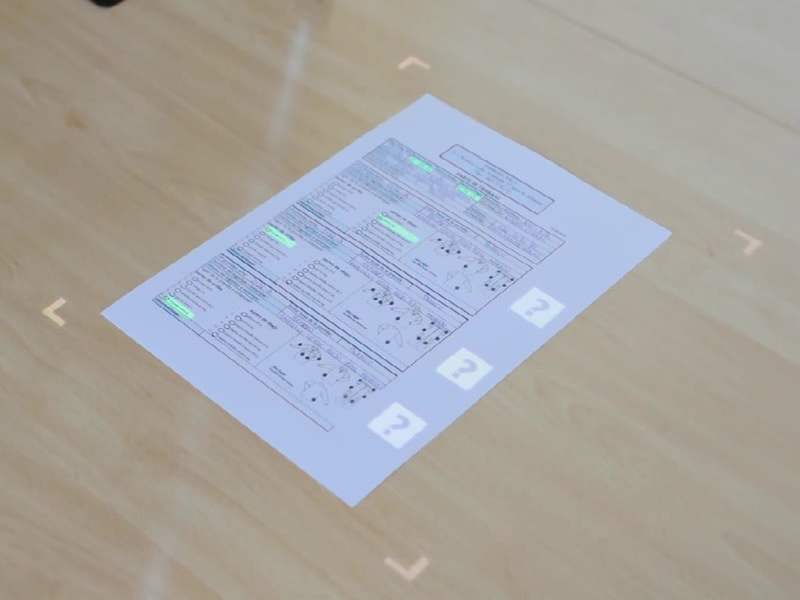
\includegraphics[width=1.0\textwidth]{ARgos_facture2.png}
    \caption{Segundo documento detectado y componentes gráficos desplegados.}
    \label{fig:ARgos_facture2}
  \end{center}
\end{figure}

\begin{figure}[!h]
  \begin{center}
    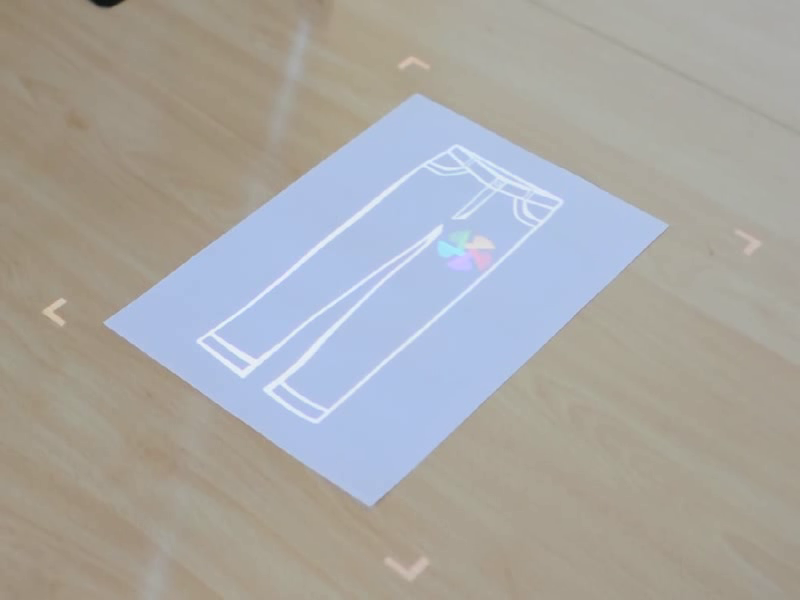
\includegraphics[width=1.0\textwidth]{ARgos_facture2_1.png}
    \caption{Segundo documento al pulsar el botón de interacción.}
    \label{fig:ARgos_facture2_1}
  \end{center}
\end{figure}

\begin{figure}[!h]
  \begin{center}
    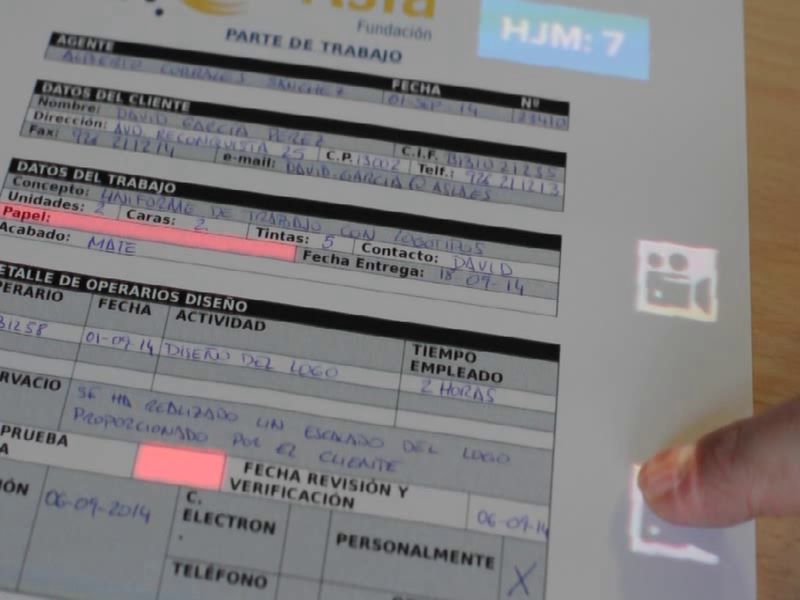
\includegraphics[width=0.9\textwidth]{pulsacion.png}
    \caption{Tercer documento detectado y componentes gráficos desplegados.}
    \label{fig:ARgos_facture3}
  \end{center}
\end{figure}

\begin{figure}[!h]
  \begin{center}
    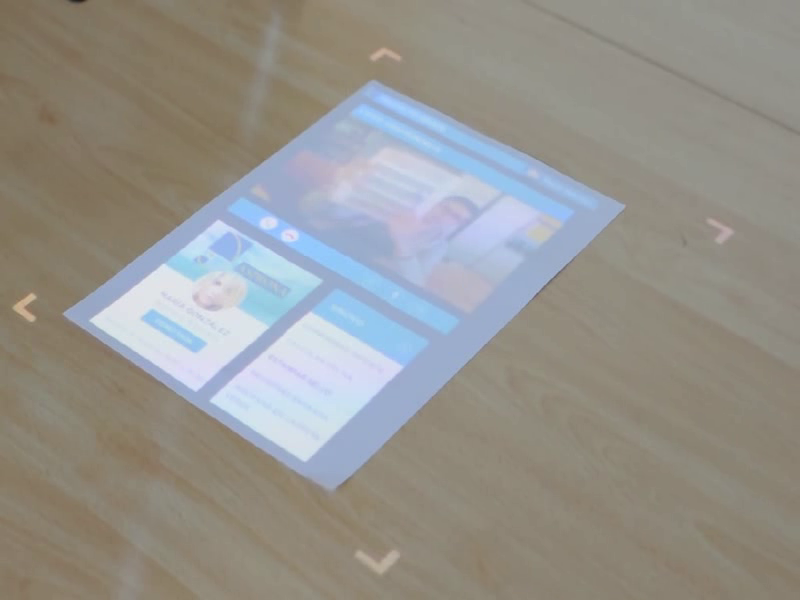
\includegraphics[width=1.0\textwidth]{ARgos_videostream2.png}
    \caption{Videollamada iniciada sobre la superficie del documento.}
    \label{fig:ARgos_videostream2}
  \end{center}
\end{figure}

\begin{figure}[!h]
  \begin{center}
    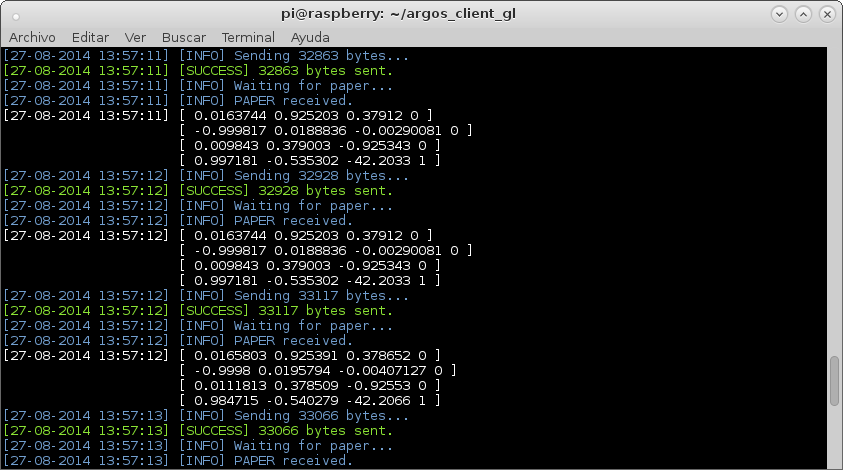
\includegraphics[width=1.0\textwidth]{Client_loop.png}
    \caption{Registro de eventos del cliente mientras se ejecuta el bucle principal del sistema.}
    \label{fig:Client_loop}
  \end{center}
\end{figure}

\begin{figure}[!h]
  \begin{center}
    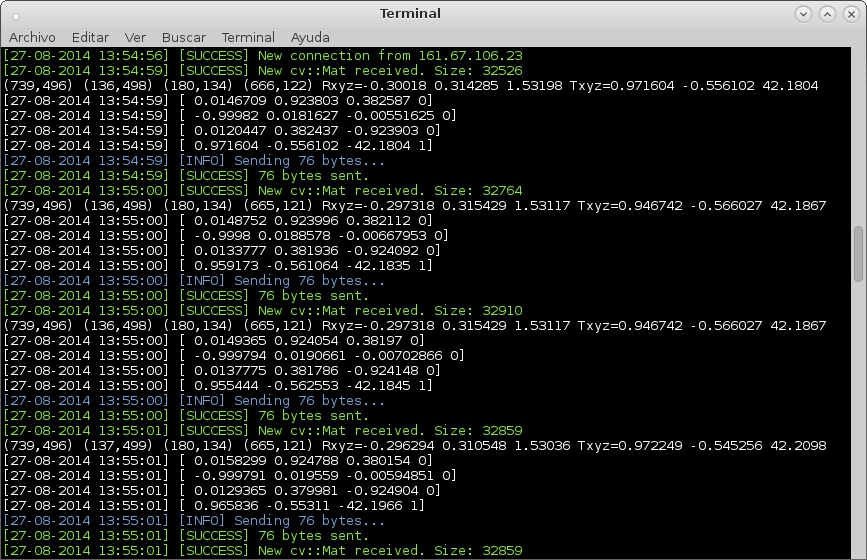
\includegraphics[width=1.0\textwidth]{Server_listening.png}
    \caption{Registro de eventos del servidor mientras se ejecuta el bucle principal del sistema.}
    \label{fig:Server_listening}
  \end{center}
\end{figure}

\begin{figure}[!h]
  \begin{center}
    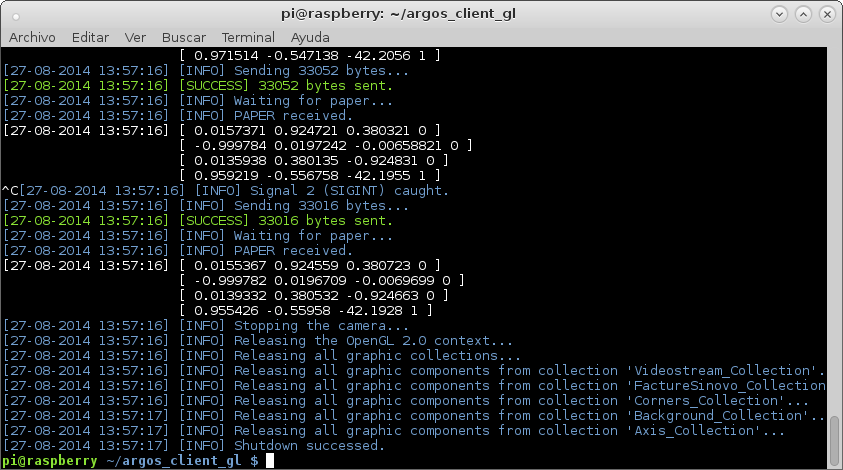
\includegraphics[width=1.0\textwidth]{Client_release.png}
    \caption{Cierre de sistemas y liberación de la memoria del cliente.}
    \label{fig:Client_release}
  \end{center}
\end{figure}

% Local Variables:
% TeX-master: "main.tex"
%  coding: utf-8
%  mode: latex
%  mode: flyspell
%  ispell-local-dictionary: "castellano8"
% End:
